% !TeX root = relazione.tex
\documentclass{article}

\usepackage[utf8]{inputenc}
\usepackage[a4paper, total={15.3 cm, 21.3 cm}]{geometry}
\usepackage{amsmath}
\usepackage{amssymb}
\usepackage{gensymb}
\usepackage{booktabs}
\usepackage{hyperref}
\usepackage{caption}
\usepackage{float}
\usepackage{graphicx}
\usepackage{subfig}
\usepackage{titlesec}
\usepackage{titletoc}
\usepackage{physics}
\usepackage{siunitx}
\usepackage[dvipsnames]{xcolor}
\usepackage{longtable}
\usepackage{calc}
\usepackage{array}
\usepackage{subfiles} % Best loaded last in the preamble
\usepackage{etoolbox}
\usepackage{xparse}

\hypersetup{colorlinks=true,linkcolor=black}
\renewcommand\thesection{\arabic{section}}
\titlecontents{chapter}[1.05em]{\bigskip}
{\contentslabel[\MakeUppercase{\romannumeral\thecontentslabel}]{1em}\enspace\textsc}
{\hspace*{-1em}\textsc}
{\hfill\contentspage}
\titlecontents{section}[1.6em]{\smallskip}
{\thecontentslabel.\enspace}
{}
{\titlerule*[1pc]{.}\contentspage}
\setcounter{tocdepth}{2}


\begin{document}

    \pagenumbering{roman}
    \thispagestyle{empty}

    \begin{center}

        
\includegraphics[width=1.\linewidth]{../../../tools/logo.jpg}
        \centering
        \vspace{3cm}
        
    {\uppercase{\Large Lab Report:\\ Interferometro di Michelson\par}}
    \vspace{3cm}
    
    {\Large Lorenzo Liuzzo, Jiahao Miao, Riccardo Salto\par}
    \vspace{1.5cm}
    
    {\Large \today}
    
\end{center}
\clearpage

\tableofcontents
\clearpage

\pagenumbering{arabic}

\section{Abstract}

In questa esperienza di laboratorio si è osservato il fenomeno dell'interferenza luminosa e misurato le seguenti quantità:
\begin{enumerate}
    \item la lunghezza d'onda $\lambda$ del laser in dotazione controllando finemente una vite micrometrica \ref{fig:apparato} e conteggiando il numero delle frange di interferenza formatosi su uno schermo.
    \item l'indice di rifrazione dell'aria $n_a$ grazie ad una cameretta sigillata ed una pompa per vuoto.
    \item la lunghezza di coerenza  della luce bianca $L_b$ e verde $L_v$osservando il fenomeno di interferenza del pacchetto d'onda su uno schermo.
    \item la separazione $\Delta\lambda$tra le due righe del doppietto della luce gialla del sodio sfruttando l'interferenza tra le due lunghezze d'onda.

    Riportiamo di seguito i valori finali ottenuti durante questa esperienza:
    \begin{align*}
         \lambda &= (632 \pm 7) \qq{nm}\\
         n_a &= 1,000265 \pm 0,000006 \\
        L_b &= (8,0 \pm 1,3)\cdot 10^{-6} m\\
        L_v &= (30,0 \pm 0,1)\cdot 10^{-6} m\\ 
         \Delta\lambda &= (5.97 \pm 0.03)10^{-10} m
    \end{align*}
    
\end{enumerate}


\section{Metodi}
\subsection{Ortogonalizzazione specchi}
    La prima fase della taratura dell'apparato è stata la regolazione degli specchi utilizzando la luce del laser: osservando su un foglio di carta gli spot luminosi dovuti alle riflessioni principali dei due specchi, è stata aggiustata con viti micrometriche (V in figura \ref{fig:apparato}) l'inclinazione dello specchio fisso S2 affinché i due coincidessero. E' poi stata inserita una lente convergente, regolata in modo da non alterare la direzione del fascio, per allargare gli spot luminosi e rendere visibili le frange di interferenza. A questo punto lo specchio S2 è stato regolato in modo da osservare meglio le frange d'interferenza. In figura \ref{fig:apparato} è riportato uno schema dell'apparato utilizzato
    \begin{figure}[h]
        \centering
        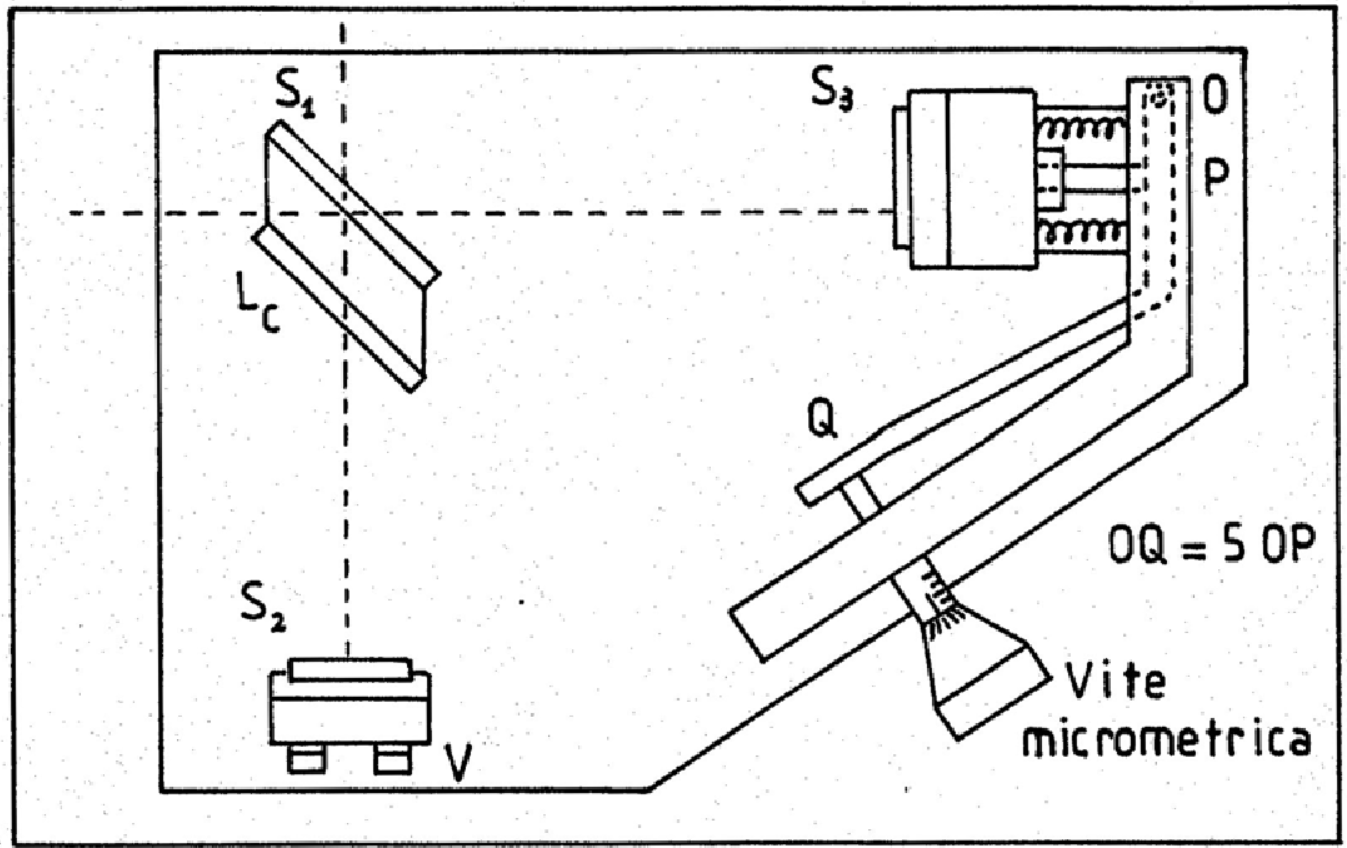
\includegraphics[scale=0.3]{../images/apparato_michelson.png}
        \caption{Schema dell'apparato sperimentale}
        \label{fig:apparato}
    \end{figure}
\subsection{Misura della lunghezza d'onda del laser}
    Per misurare la lunghezza d'onda del laser utilizzato nella fase di calibrazione sono state contate le fasce di interferenza che venivano prodotte spostando lo specchio S3 di una distanza nota. Per avere una misura più accurata i conteggi delle frange sono stati effettuati da due persone per volta, il risultato è stato mediato e come errore associato è stata presa la deviazione standard. Lo spostamento dello specchio è stato invece misurato come differenza tra la posizione iniziale e quella finale utilizzando un micrometro con risoluzione $0.01$mm collegato a una leva che ne quintuplica la precisione fino a $0.002$ mm. L'errore però è stato considerato sottostimato dato che non tiene conto dei possibili giochi tra le componenti meccaniche del carrello su cui si muove S3. Per questo motivo si è scelto di associare un errore sistematico di $\pm 0.001$mm, ottenendo quindi come incertezza associata ad ogni misura di posizione $0.003$ mm. Sono state effettuate 5 misure delle quali in \ref{misure laser} sono riportati lo spostamento di S3 $\Delta$x, la media del numero di frange contate dai due osservatori  $N_{medio}$ e il valore della lunghezza d'onda ricavato indirettamente dalle due misure precedenti $\lambda$.


    
     \begin{table}[H]
        \begin{minipage}[b]{0.35\linewidth}
            \begin{tabular}{ ccc } 
                \toprule 
                $\Delta$x [m] & $N_{medio}$ & $\lambda$ [m] \\
                \midrule 
                6,20E-05 & 197 & 6,29E-07 \\
                6,80E-05 & 216 & 6,31E-07 \\
                6,40E-05 & 201 & 6,37E-07 \\
                7,00E-05 & 220 & 6,36E-07 \\
                7,80E-05 & 249 & 6,28E-07 \\
                \bottomrule           
            \end{tabular}
            \caption{misure $\lambda$ laser}
            \label{misure laser}
            \end{minipage}
            \begin{minipage}[b]{0.65\linewidth}
            \centering
                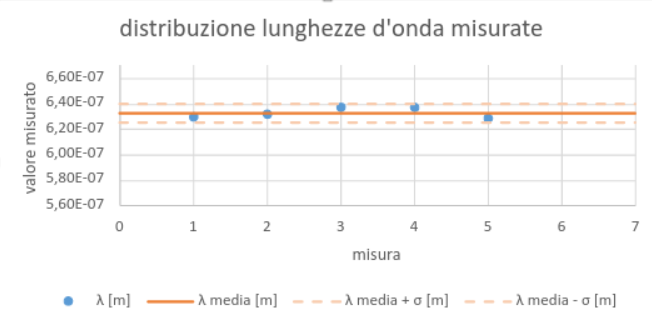
\includegraphics[scale = 0.4]{../images/graph_laser.png}
                
                \captionof{figure}{Grafico distribuzione delle misure della lunghezza d'onda del laser ottenuto}
                \label{graph:laser}
                
            \end{minipage}
        \end{table}

        
    Il valore della lunghezza d'onda del laser $\lambda$ è stato ottenuto tramite la relazione:
        \[\lambda = \frac{2n_a\Delta x}{N_1}\]
    dove $n_a$, indice di rifrazione dell'aria, è stato approssimato a 1. Gli errori associati alle lunghezze d'onda $\sigma_{\lambda}$ sono invece stati stimati con la seguente formula di propagazione:
    \begin{align*}
        \sigma_{\lambda} &= 2 \frac{n_{a}}{N_{medio}} \sqrt{(\sigma_{N_{medio}}\frac{\Delta x }{N_{medio}})^2 + (\sigma_{\Delta x})^2}\\
        &= |\lambda|\cdot \sqrt{(\frac{\sigma_{N_{medio}} }{N_{medio}})^2 + (\frac{\sigma_{\Delta x}}{\Delta x})^2}
    \end{align*}
    
    Dove
    \begin{itemize}
        \item $\sigma_N$ è l'errore associato al conteggio delle frange stimato come la deviazione standard tra i due valori ottenuti,
        \item  $\sigma_{\Delta x}$ è invece l'errore associato allo spostamento di S3, stimato come somma in quadratura degli errori associati alla singola misura di posizione ($0.004$ mm).
    \end{itemize}
    
    Dalla propagazione gli errori sono risultati uniformi per tutte e cinque le misure e valutabili come: 
        \[\sigma_{\lambda}= 2\ 10^{-8}\ m\]
    Il valore finale, ottenuto da una media pesata dei valori in tabella, è: 
        \[\lambda = (632 \pm 7) \qq{nm}\]

    \subsection{Misura dell'indice di rifrazione dell'aria}
    
        Per quanto riguarda la misura dell'indice di rifrazione dell'aria è stata utilizzata una camera sigillata dove poteva essere creato il vuoto con una pompa elettrica. La lunghezza della camera $d$ è stata stimata $5$ cm e ad occhio è stata considerata la presenza di guarnizioni e la posizione effettiva delle finestre trasparenti per cui è stato considerato un errore di $0.2$ mm. A questo punto è stato creato il vuoto con la pompa. Aprendo la valvola in modo da permettere un lento rifluire dell'aria e contando il numero di frange $N_f$ di interferenza che passavano sullo schermo è stato stimato l'indice di rifrazione $n_{aria} $attraverso la relazione:
             \[n_{aria}  = \frac{N_f\lambda}{2d}+1\]

        Nota $\lambda$, lunghezza d'onda del laser, calcolata nella parte precedente dell'esperimento. Il valore di $N_f$ è stato stimato con una media tra i due valori ottenuti dagli osservatori come è stato fatto nella parte precedente dell'esperimento, la sua incertezza $\sigma_N$ è la deviazione standard delle misure.  Per quanto guarda gli errori sulle misure dell'indice di rifrazione $\sigma_n$ è stata invece usata la seguente relazione di propagazione:

        \begin{align*}
            \sigma_{n_a} &= \frac{1}{2d} \sqrt{(\sigma_{N_f} \lambda)^2+(\sigma_{\lambda} N_f)^2+(\frac{\sigma_d N_f \lambda}{d} )^2 }\\
            &= \frac{\lambda N_f}{2d} \sqrt{(\frac{\sigma_{N_f}}{N_f} )^2+(\frac{\sigma_{\lambda}}{\lambda})^2+(\frac{\sigma_d}{d} )^2 }\\
            &=|n_a -1 | \cdot \sqrt{(\frac{\sigma_{N_f}}{N_f} )^2+(\frac{\sigma_{\lambda}}{\lambda})^2+(\frac{\sigma_d}{d} )^2 }
        \end{align*}
          
        Dove
        \begin{itemize}
            \item $\sigma_{N_f}$ è l'incertezza sul conteggio, stimato come deviazione standard tra i due conteggi.
            \item $\sigma_{\lambda}$ è l'incertezza sul valore della lunghezza d'onda del laser, calcolato precedentemente ($5$ nm).
            \item $\sigma_d$ è l'incertezza sulla lunghezza della cameretta, stimato con buonsenso.
        \end{itemize}
         Le incertezze sono risultate uniformi per tutte le misure, con valore: 
            \[\sigma_n \approx 1\cdot10^{-5}\]
        La misura è stata ripetuta 5 volte; in tabella \ref{misure: n aria} sono riportati il numero di frange medio $N_f$ e il valore dell'indice di rifrazione associato $n_{aria}$.
        \begin{table}[H]
        \begin{minipage}[b]{0.35\linewidth}
        \centering
            \begin{tabular}{ cc } 
                \toprule 
                 $N_{f}$ & $n_{aria}$  \\
                \midrule 
                42 & 1,000265 \\
                43 & 1,000268\\
                42 & 1,000262\\
                41 & 1,000259\\
                43 & 1,000268\\
                \bottomrule           
            \end{tabular}
            \caption{misure $n_{aria}$}
            \label{misure: n aria}
            \end{minipage}
            \begin{minipage}[b]{0.65\linewidth}
                    \centering
                    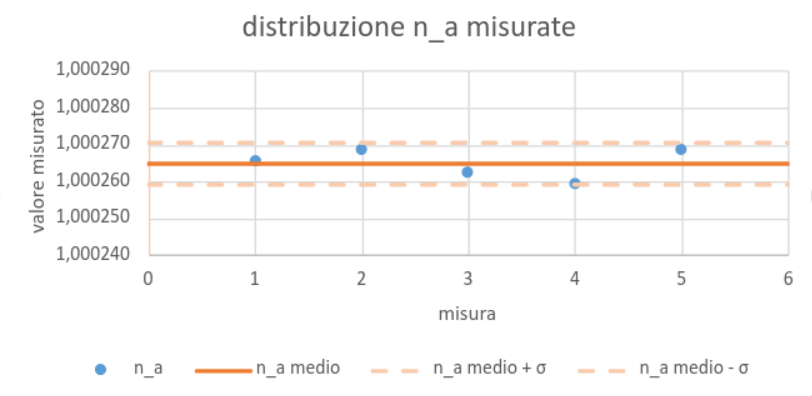
\includegraphics[scale=0.3]{../images/graph_n_a.png}
                    \caption{Distribuzione delle indici di rifrazione}
                    \label{graph: Indici di rigrazione}
            \end{minipage}
        \end{table}
        
        Con una media pesata è stato ottenuto il valore finale:
            \[n_a = 1,000265 \pm 0,000006\]
            
\subsection{Misura della lunghezza del pacchetto d'onda della luce bianca e verde}
    Per misurare la lunghezza di un pacchetto d'onda di luce bianca è stato necessario pareggiare la lunghezza dei bracci dell'interferometro con una precisione dell'ordine dei $5\ \mu$m. Per semplificare la procedura è stato utilizzato ancora il laser: dopo aver modificato l'inclinazione di $S2$ (vedi figura \ref{fig:apparato})in modo da far apparire sullo schermo linee il più possibile rette, è stata fatta variare la posizione di $S3$ in modo da osservare il range entro il quale queste passavano da concavità verso l'alto a concavità verso il basso. A questo punto, una volta sostituito il laser con la lampada a incandescenza, $S3$ è stato fatto variare nel range trovato fino a che non sono state osservate le bande di interferenza di un pacchetto d'onda. Con il micrometro è stata misurata la posizione in cui si è iniziata a vedere l'interferenza e quella a cui è scomparsa. La differenza tra le due posizioni sarebbe stata proprio la grandezza cercata. Sono state effettuate 5 misure.
    La stessa procedura è stata ripetuta schermando la lampada a incandescenza con un filtro verde. In tabella \ref{misure: pacchetto d'onda luce bianca e verde} sono riportati i valori misurati di lunghezza del pacchetto d'onda di luce bianca $\Delta x_{bianco}$ e verde $\Delta x_{verde}$.
    \begin{table}[H]
    \begin{minipage}[b]{0.35\linewidth}
        \centering
            \begin{tabular}{ cc } 
                \toprule 
                 $\Delta x_{bianco}$[m] & $\Delta x_{verde}$[m]  \\
                \midrule 
                8E-06	&	3,20E-05 \\
                8E-06	&	3,20E-05\\
                8E-06	&	3,00E-05\\
                8E-06	&	2,80E-05\\  
                8E-06	&	3,00E-05\\
                \bottomrule           
            \end{tabular}
            \caption{misure pacchetti d'onda luce bianca e verde}
            \label{misure: pacchetto d'onda luce bianca e verde}
        \end{minipage}
        \begin{minipage}[b]{0.65\linewidth}
                \centering
                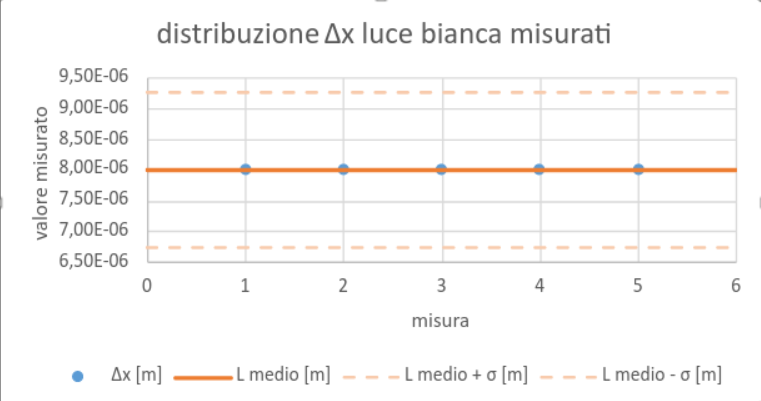
\includegraphics[scale=0.3]{../images/luce_bianca.png}
                \caption{Distribuzione delle misure di lunghezza del pacchetto d'onda della luce bianca}
                \label{graph:luce bianca}
        \end{minipage}
        
        \end{table}
    Avendo effettuato una misura diretta della lunghezza dei pacchetti d'onda prendendo la differenza di posizione di S3 tra inizio e fine del pacchetto, si è associato come errore sulla misura $\sigma_{\Delta x}$ la somma in quadratura delle incertezze legate alle singole misure di posizione ($0.003$ mm), il cui valore è:
        \[\sigma_{\Delta x} = 3\cdot10^{-6} m \]
    Con una media aritmetica è stato trovato il valore finale di lunghezza dei pacchetti di luce bianca $L_b$ e verde $L_v$:
    \begin{align*}
        L_b &= (8,0 \pm 1,3)\cdot 10^{-6} m\\
        L_v &= (30,0 \pm 0,1)\cdot 10^{-6} m\\ 
    \end{align*}
        
    Associando a tutte le misure la stessa incertezza, in questo caso la media pesata coincide con la media aritmetica. L'incertezza finale è dato dall'incertezza diviso la radice del numero di misure effettuate.
    \[\frac{\sigma_{\Delta x}}{\sqrt{5}}\]
\subsection{Misura della differenza di lunghezza d'onda del doppietto del sodio}
    La seguente misura è stata effettuata, dopo aver posizionato la lampada ai vapori di sodio in modo che la luce emessa fosse centrata con l'apparato, spostando $S3$, vedi figura \ref{fig:apparato}, con il micrometro e osservando a che altezza comparisse un'unica figura luminosa corrispondente alla configurazione nella quale le frange luminose della prima riga del doppietto del sodio si sovrappongono alle frange scure della seconda. Variando la posizione di $S3$ è stata misurata la distanza tra una, due o tre figure luminose. 
    Attraverso la relazione:
        \[\Delta \lambda = \frac{m \lambda^2}{2\Delta x}\]
    è stata stimata la differenza di lunghezze d'onda emesse dalla lampada a vapori di sodio $\Delta \lambda$, dove $\lambda$ è il valore medio delle lunghezze d'onda note del doppietto del sodio la cui incertezza è trascurabile, $m$ è il numero di alternanze luminose di cui si vuole misurare la distanza e $\Delta x $ è la differenza tra le posizioni di inizio condizione di interferenza netta e l'm-esimo inizio condizione di interferenza netta misurata con il micrometro, la cui incertezza $\sigma_{\Delta x}$ è stata valutata come somma in quadratura delle incertezze associate alla singola misura di posizione (che si ricorda essere stata stimata $0.003$mm). In Tabella \ref{misure: doppietto sodio} sono riportati i valori delle distanze, il numero di alternanze luminose e la differenza di lunghezze d'onda misurata a partire da queste con relativa incertezza $\sigma_{\Delta\lambda}$ calcolato dalla relazione:
        \[\sigma_{\Delta\lambda}= \Delta\lambda \frac{\sigma_{\Delta x}}{\Delta x}\]
    Il valore migliore ottenuto con una media pesata è: 
        \[\Delta\lambda= (5.97 \pm 0.03)10^{-10} m\]
    \begin{table}[H]
     \begin{minipage}[b]{0.35\linewidth}
        \centering
            \begin{tabular}{ cccc } 
                \toprule 
                $\Delta$ x [m] & $N_{passi}$ & $\Delta\lambda$ [m] &$ \sigma_{\Delta\lambda}$ \\
                \midrule 
                0,00030	&	1	&	5,78791E-10	&	2E-11	\\
                0,00060	&	2	&	5,78791E-10	&	9E-12	\\
                0,00086	&	3	&	6,02907E-10	&	6E-12	\\
                0,00086	&	3	&	6,02907E-10	&	6E-12	\\
                0,00087	&	3	&	5,98749E-10	&	6E-12	\\
                \bottomrule           
            \end{tabular}
            \caption{misure distanza doppietto del sodio}
           \label{misure: doppietto sodio}
           \end{minipage}
           \begin{minipage}[b]{0.65\linewidth}
                   \centering
                   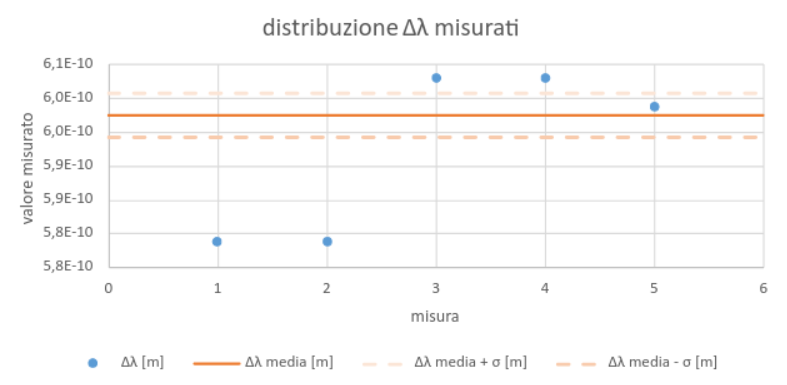
\includegraphics[scale= 0.3]{../images/doppietto_sodio.png}
                   \caption{Distrubuzione delle misure della separazione tra le righe del doppietto del sodio}
                   \label{fig:my_label}     
           \end{minipage}
        \end{table}


\end{document}
